\documentclass[a4paper, table]{article}
\input{General/Preamble} % Loads in the preamble 
% Give your report a title
\newcommand\reporttitle{Project}

% Insert course code, name, quartile number and year (or any other subtitle)
\newcommand\reportsubtitle{
BCS1110, Introduction to Computer Science
}

% Add your group number (for DBL) or any other text.
\newcommand\groupnumber{
\textbf{Group 11}
}

% Insert authors and student numbers here
\newcommand\reportauthors{
Long Luong & I6359380\\
Élisa Donéa & I6356213\\
Chris Munteanu & I6344912\\
Alexia Raportaru & I6355814\\
}

% Add the name of your tutor (for DBL) or any other text.
\newcommand\grouptutor{
Professors: Dr. Ashish Sai, Dr. Thomas Bitterman
}

% Date and location (default: current date and Eindhoven)
\newcommand\placeanddate{
Maastricht, \today
}

% Define Tue-red (color of the TU/e logo). Can be changed to drastically change the look of the template
\definecolor{Tue-red}{RGB}{0, 25, 58}

% All of the following code can be removed to be left with (close to) default LaTeX behaviour. 

% Sets up hyperlinks in the document to be colored
\hypersetup{
    colorlinks=true,
    linkcolor=Tue-red,
    urlcolor=Tue-red,
    citecolor = Tue-red
    }
\urlstyle{same} % Defines settings for link and reference formatting


% Change bullet style for level 1, 2 and 3 respectively for itemize
\renewcommand{\labelitemi}{\scriptsize\textcolor{Tue-red}{$\blacksquare$}}% level 1
\renewcommand{\labelitemii}{\scriptsize\textcolor{Tue-red}{$\square$}}% level 2
\renewcommand{\labelitemiii}{\textcolor{Tue-red}{$\circ$}}% level 3

% \renewcommand{\labelitemi}{\small\textcolor{Tue-red}{\ding{70}}} % level 1
% \renewcommand{\labelitemii}{\small\textcolor{Tue-red}{\ding{71}}}% level 2
% \renewcommand{\labelitemiii}{\tiny\textcolor{Tue-red}{\ding{71}}}% level 3

% Change bullet style for level 1, 2 and 3 respectively for enumerate
\renewcommand{\labelenumi}{\textbf{\textcolor{Tue-red}{\arabic*.}}}% level 1
\renewcommand{\labelenumii}{\textbf{\textcolor{Tue-red}{[\alph*]}}}% level 2
\renewcommand{\labelenumiii}{\textbf{\textcolor{Tue-red}{\roman*.}}}% level 3

% Have reference labels be linked to section (section 3 will have fig. 3.1 etc.)
\counterwithin{equation}{section} % For equations
\counterwithin{figure}{section} % For figures
\counterwithin{table}{section} % For tables

% Creates a beautiful header/footer
\pagestyle{fancy}
\lhead{\includegraphics[height = 16pt]{Figures/0. General/maastricht-logo-wide.png}}
\rhead{\reporttitle}
\renewcommand{\footrulewidth}{0.4pt}
\cfoot{Page \thepage}

% Formats section, subsection and subsubsection titles respectively 
\titleformat{\section}{\sffamily\color{Tue-red}\Large\bfseries}{\thesection\enskip\color{gray}\textbar\enskip}{0cm}{} % Formats section titles

\titleformat{\subsection}{\sffamily\color{Tue-red}\large\bfseries}{\thesubsection\enskip\color{gray}\textbar\enskip}{0cm}{} % Formats subsection titles

\titleformat{\subsubsection}{\sffamily\color{Tue-red}\bfseries}{\thesubsubsection\enskip\color{gray}\textbar\enskip}{0cm}{} % Formats subsubsection titles

% Formats captions
\DeclareCaptionFont{Tue-red}{\color{Tue-red}}
\captionsetup{labelfont={Tue-red,bf}}

 % Changes font to mlmodern
\usepackage{mlmodern}

% Removes indent when starting a new paragraph
\setlength\parindent{0pt}

% Limits the ToC to sections and subsections (no subsubsec.)
\setcounter{tocdepth}{2}
 % Loads in user defined settings
\begin{document}

% Inserts the front page
\input{Chapters/0. Frontpage}
\newpage

% Generates a ToC without page number
{\hypersetup{linkcolor=black} % Keeps the ToC black even with non-black linkcolor
\tableofcontents\thispagestyle{empty}}
\newpage

% contains inspiration for formatting tables, images, text citations etc.
% \input{Chapters/Z. Template} % Feel free to remove / comment out
% \newpage

% Creates the introduction, starting page numbering
\section{Introduction} \label{section: introduction}
JavaCraft is a a multifaceted text-based Java game inspired by Minecraft. The game is a relatively complex Java program that brings over 35 functions to create a diverse gameplay experience. This team project is an academic exercise in computer science, logical thinking, and collaboration. Working in teams of four, we used our creativity, analytical skills, and technical skills to analyse and expand upon the existing JavaCraft game. The source code of JavaCraft can be found in the following link: \url{https://gitlab.maastrichtuniversity.nl/bcs1110/javacraft/-/raw/main/JavaCraft.java} \\

Below is a table that describes what each team member did on the project, divided by section:

\begin{center}
    \begin{tabular}{ l l }
     Section & Who did what\\
     \hline
     Introduction & Long (100\%)\\  
     JavaCraft's Workflow & Alexia (100\%) \\
     Functionality Exploration & Long (60\%), Élisa (40\%) \\
     Secret Door FSA Design & Élisa (50\%), Chris (50\%) \\
     Git Collaboration \& Version Control & Alexia (25\%), Élisa (25\%), Chris (25\%), Long (25\%) \\
     Extending the Game Code & Alexia (35\%), Long (65\%) \\
     Interacting with Flags API & Élisa (50\%), Chris (15\%), Long (35\%) \\
     Report & Long (100\%) \\ 
    \end{tabular}
\end{center}
 \pagenumbering{arabic}
\newpage

\section{JavaCraft's Workflow} \label{section: javacraft workflow}
In order to fully understand the mechanism of the game, a flowchart of the entire game is provided below. The flowchart is accompanied by pseudocode.

Insert flowchart of game
Insert pseudocode for game

\newpage

\section{Functionality Exploration} \label{section: functionality exploration}

This section describes several functions found in the JavaCraft.java file. Out of the functions, there are fifteen who have a flowchart and pseudocode.

\begin{table}[ht]
    \rowcolors{2}{gray!10}{white}
    \centering
    \caption{A table that describes functions used in javacraft}
    \begin{tabular}{ccc}
    \toprule
    \textbf{No.}&\textbf{Function Name}&\textbf{Description}\\
    \midrule
    1& \texttt{void generateWorld} & assigns integer to every tile of the world\\
    2& \texttt{void initGame} & \makecell{creates world with width \texttt{worldWidth} \\and height \texttt{worldHeight}}\\
    3& \texttt{void main} & main function\\
    4& \texttt{void startGame} & starts the game\\
    5& \texttt{void movePlayer} & moves player horizontally or vertically\\
    6& \texttt{void mineBlock} & mines block player is on if block is not air\\
    7& \texttt{String getBlockSymbol} & returns symbol of \texttt{blockType}\\
    8& \texttt{void resetWorld} & clears the world and sets player position in middle\\
    9& \texttt{void generateEmptyWorld} & generates an empty world\\
    10& \texttt{void clearScreen} & clears terminal\\
    11& \texttt{void lookAround} & prints out adjacent squares to player\\
    12& \texttt{void fillInventory} & completely fills up inventory of player\\
    13& \texttt{void displayLegend} & displays a legend of what each tile represents\\
    14& \texttt{void displayWorld} & prints out all tiles of the world\\
    15& \texttt{void displayInventory} & prints out obtained items \& crafted items\\
    16& \texttt{void loadGame} & loads the game from file \texttt{fileName}\\
    17& \texttt{void saveGame} & saves the game in file \texttt{fileName}\\
    18& \texttt{void interactWithWorld} & interacts with item player is standing on\\
    19& \texttt{void addCraftedItem} & adds item \texttt{craftedItem} to array \texttt{craftedItems} \\
    20& \texttt{void removeItemsFromInventory} & removes item \texttt{item} \texttt{count} times from inventory\\
    21& \texttt{boolean inventoryContains} & returns boolean of whether \texttt{item} is in inventory\\
    22& \texttt{void placeBlock} & places block \texttt{blockType} at player position\\
    23& \texttt{void displayCraftingRecipes} & prints out available crafting recipes\\
    24& \texttt{void craftItem} & crafts an item based on argument \texttt{recipe}\\
    25& \texttt{void craftIronIngot} & crafts an iron ingot\\
    26& \texttt{void craftStick} & crafts a stick\\
    27& \texttt{void waitForEnter} & waits for operator to press Enter\\
    28& \texttt{String getBlockTypeFromCraftedItem} & returns integer of \texttt{craftedItem}\\
    29& \texttt{String getCraftedItemFromBlockType} & returns integer of \texttt{blockType}\\
    30& \texttt{String getBlockName} & returns name of \texttt{blockType}\\
    31& \texttt{String getBlockColor} & returns color of \texttt{blockType}\\
    32& \texttt{String getCraftedItemName} & returns name of \texttt{craftedItem}\\
    33& \texttt{String getCraftedItemColor} & returns color of \texttt{craftedItem}\\
    34& \texttt{char getBlockChar} & returns char of \texttt{blockType}\\
    35& \texttt{void craftWoodenPlanks} & crafts wooden planks\\
    36& \texttt{void getCountryAndQuoteFromServer} & \makecell{makes HTTP request and writes data \\ to server and prints country and quote}\\
    \bottomrule
    \end{tabular}
    \label{table: style 2}
\end{table}
\newpage

\section{Finite State Automata (FSA) Design} \label{section: fsa design}
The following describes the Secret Door Logic through an FSA illustration and a description: \\

We have 18 finite set of states and in our alphabet we have "open" , "wasd", "c", "m" and "unlock" 
On step one Q0 you have to write unlock if not you will remain in Q0
After you have arrived in Q1 you have the choice in between wasd, c, m because in able to unlock the secret door you must c, craft then m, mine or wasd to move in any order that's why after Q1 it divides in 3 because the order is not important.
If you type a move command (w,a,s or d) you enter Q2, the only options you have from now are mine or craft if not you stay in Q2 unless you type open which sends you back to Q0 and have to start again. If you type c you go into Q3 so the last thing you have to write is mine if you write anything else you stay in Q3 expect "open" which sends you in Q0 after mining you enter Q4. From there your only option is to "open" which unlocks the secret door.
Now because the order doesn't matter after Q2  you can also type m for mine which sends you in Q5 where the only option is c, "craft" if you type anything else you go back to Q0 after you type C you entre Q6 where you can only type "open" which will unlock the secret door.
We have created 2 other branches based on the same principal so we can cover all the possible ways you can access the secret door

Note: in our alphabet "wasd" stands for "w", "a", "s" or "d" 

{\includegraphics[width=\textwidth,height=\textheight,keepaspectratio]{../dfa.png}}

\newpage

\section{Git Collaboration \& Version Control} \label{section: git}
The link to the JavaCraft branch can be found here: \href{https://gitlab.maastrichtuniversity.nl/bcs1110/javacraft/-/tree/group11}{https://gitlab.maastrichtuniversity.nl/bcs1110/javacraft/-/tree/group11} \\

All the files of the project can be found in the repository. \\ 
Everything was done on one branch called group11. There were no conflicts during the process due to the way we divided the tasks. Each section of the report is done at most by two different people, with the exception of the 15 flowcharts with pseudocode. \\
For the 15 flowcharts with pseudocode, we created two folders in the git branch: one for flowcharts and one for pseudocode. The folder contains one file for each function, meaning that in total we have 15 (or more) files per folder. Having everything separated in folders makes it easy to add the files to this document and to also keep track of each other's progress.
\newpage

% \section{Team Overview} \label{section: overview}
Below describes what each team member did on the project:

\subsection{Long Luong} 
Project leader \\
LaTeX Document owner and composer \\
Created 1 flowchart with pseudocode: \\
1. getCountryAndQuoteFromServer \\
Finalised the Function Exploration part \\
Helped others with git issues \\
Refined some pseudocode that others have made

\subsection{Élisa Donéa}

Designed FSA for secret door with Chris \\
Initiated with the Function Exploration \\
Create 5 flowcharts with pseudocode: \\
1. fillInventory \\
2. generateEmptyWorld \\
3. generateWorld \\
4. initGame \\
5. lookAround \\

\subsection{Chris Munteanu}

Designed FSA for secret door with Élisa \\
Create 5 flowcharts with pseudocode: \\
1. displayInventory \\
2. getBlockName \\
3. loadGame \\
4. removeItemsFromInventory \\
5. saveGame \\

\subsection{Alexia Raportaru}

Create 5 flowcharts with pseudocode: \\
1. placeBlock \\
2. craftItem \\
3. interactWithWorld \\
4. mineBlock \\
5. movePlayer \\
Created an impressive flowchart of the entire game along with its pseudocode explanation

\subsection{Explanation}

When we first met up with each other we were with the three of us. During the first week we got to know each other. Long proposed to be the document manager because he knows how to use LaTeX. He also created a (now deprecated) GitLab repository found at \url{https://gitlab.maastrichtuniversity.nl/I6359380/test-project/}. \\
During the second week Alexia joined the group. We met up with each other and we divided the roles. We had to create at least 16 flowcharts alongside with pseudocode. Long mentioned that most of the functions are vey easy to understand, and since he wanted a difficult one he proposed to do the function getCountryAndQuoteFromServer and he proposed the other three group members to do 5 flowcharts with their respective pseudocode. Everybody agreed and thinks it is a good idea. \\
In week 3 and later Élisa and Chris decided to work on the FSA together. Everybody in the group was new to Git except Long, so he helped out everyone set-up the Git environment and he explained to everyone how it works.  In the meantime, Alexia worked on the flowchart and the pseudocode of the entire game JavaCraft. Later, Long found out he made a mistake and that we had to create a branch on the repository \url{https://gitlab.maastrichtuniversity.nl/bcs1110/javacraft/} so he informed everybody about the mistake and that we all had to migrate to the correct branch.
% \newpage

% Creates references using the Biblatex 
\bibliographystyle{plain}
\bibliography{General/References.bib}
\nocite{*}
\newpage

\appendix % Any section after this command will have a letter as an index

% Adds an appendix entry
\section{Appendix: pseudocode and flowcharts} \label{section: appendix}
This appendix provides the full blocks of pseudocode and its flowcharts.

{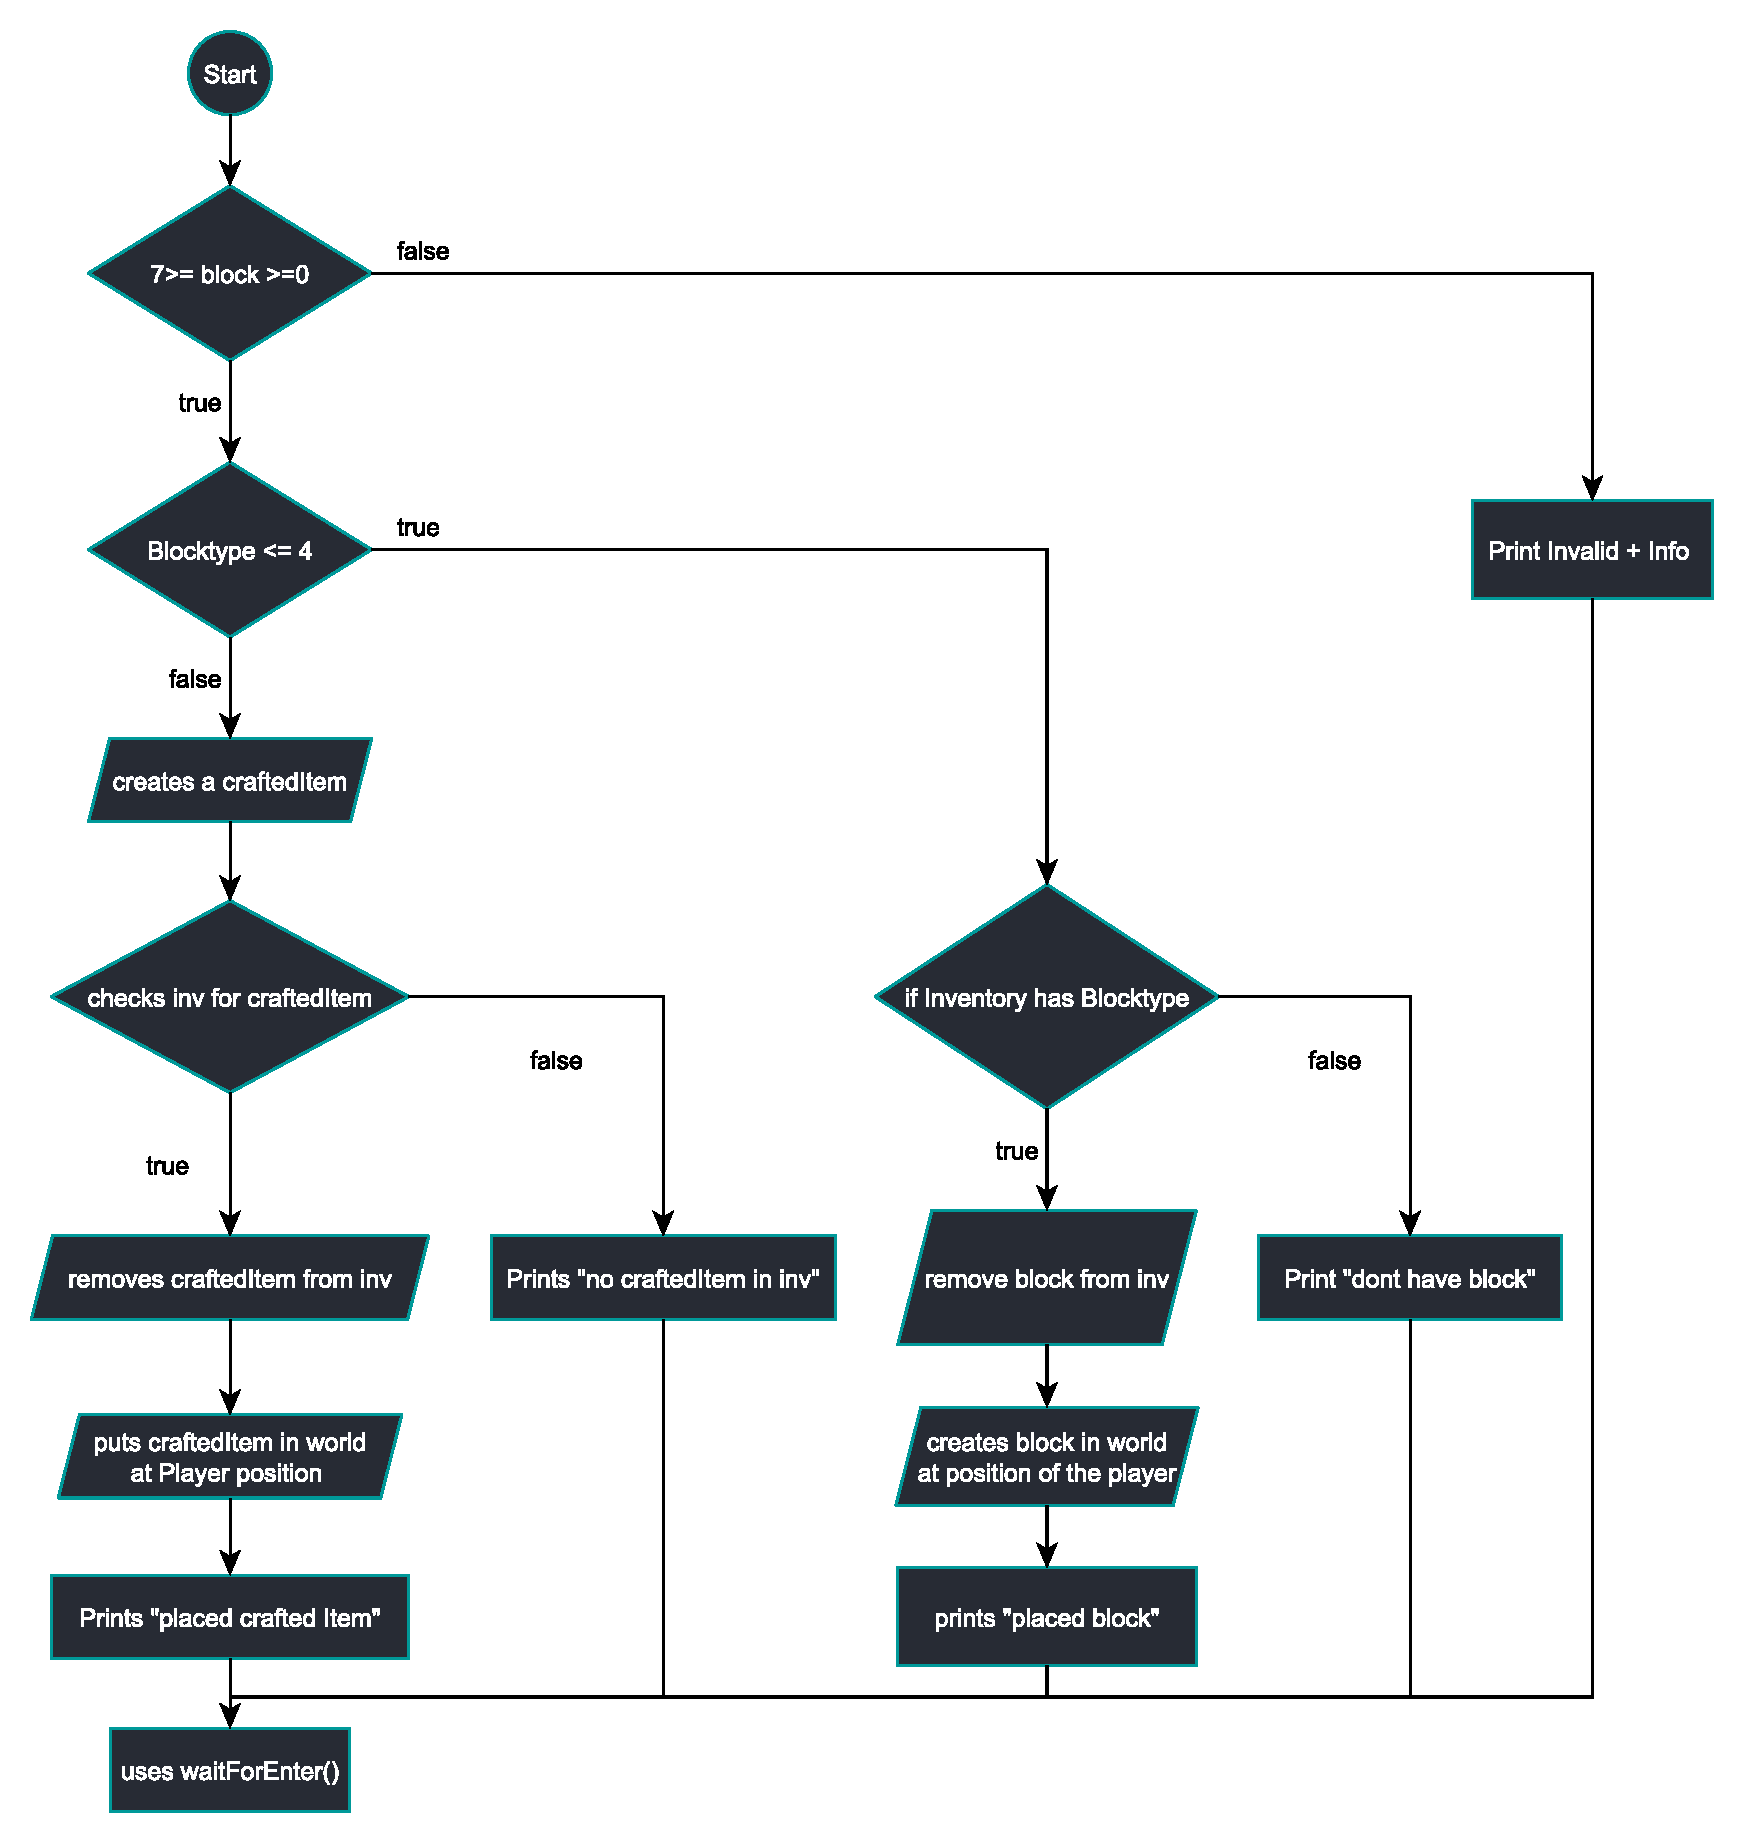
\includegraphics[width=\textwidth]{../flowchart/placeBlock.png}}

\begin{lstlisting}
function placeBlock(blockType)

if blockType is greater than or equal to 0 and blockType is less than or equal to 7 then 
	if blockType less than or equal to 4 then
		if inventory contains blockType then
			inventory.remove(blockType)
			world[playerX][playerY] = blockType
			print("Placed" + getBlockName(blockType) + " at your position.")

		else print("You don't have " + getBlockName(blockType) + " in your inventory")
		end if
	else
		craftedItem = getCraftedItemFromBlockType(blockType)
		if craftedItems contains craftedItem then 
			craftedItems.remove(craftedItem)
			world[playerX][playerY] = blockType
			print("Placed" + getCraftedItemName(craftedItem)+ " at your position.")
		else print("You don't have " + getCraftedItemName() + " in your inventory.")
		end if
	end if
else print("Invalid block number. Please enter a valid block number.")
print(BLOCK_NUMBERS_INFO)
end if
waitForEnter()
end function
\end{lstlisting}
\newpage

{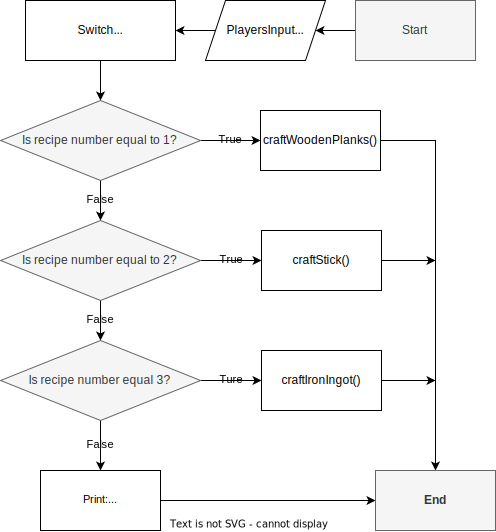
\includegraphics[width=\textwidth]{../flowchart/craftItem.png}}
\begin{lstlisting}
function craftItem(recipe)

switch(recipe)
case 1: 
	craftWoodenPlanks()
end if
case2: 
	craftStick()
end if
case3:
	craftIronIngot()
end if
default: 
	print("Invalid recipe number.")
end switch
waitForEnter()
end function
\end{lstlisting}
\newpage

{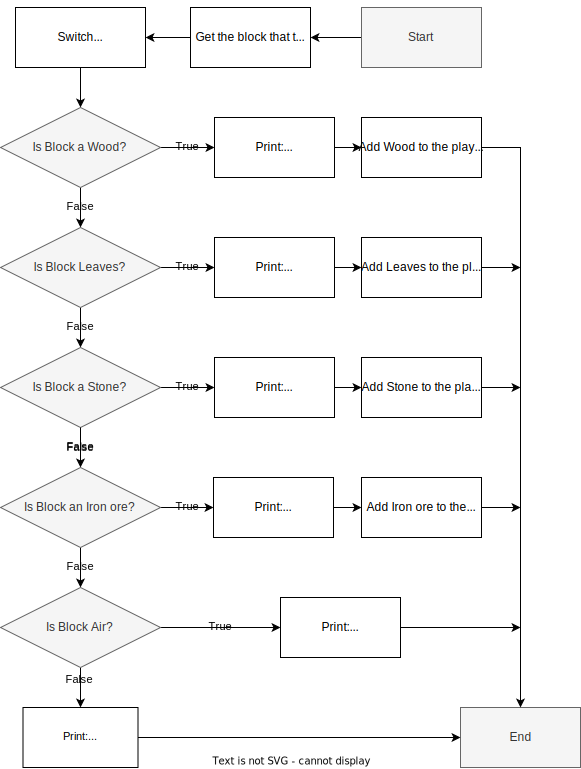
\includegraphics[width=\textwidth]{../flowchart/interactWithWorld.png}}


\begin{lstlisting}
function interactWithWorld()

blockType = world[playerX][playerY]
switch(blockType):
case WOOD: 
	print("You gather wood from the tree.")
	inventory.add(WOOD)
end if
case LEAVES:
	print("You gather leaves from the tree.")
	inventory.add(LEAVES)
end if
case STONE:
	print("You gather stones from the ground.")
	inventory.add(STONE)
end if
case IRON_ORE:
	print("You mine iron ore from the ground.")
	inventory.add(IRON_ORE)
end if
case AIR:
	print("Nothing to interact with here.")
end if
default: print("Unrecognized block. Cannot interact.")
end switch
waitForEnter()
end function
\end{lstlisting}
\newpage

{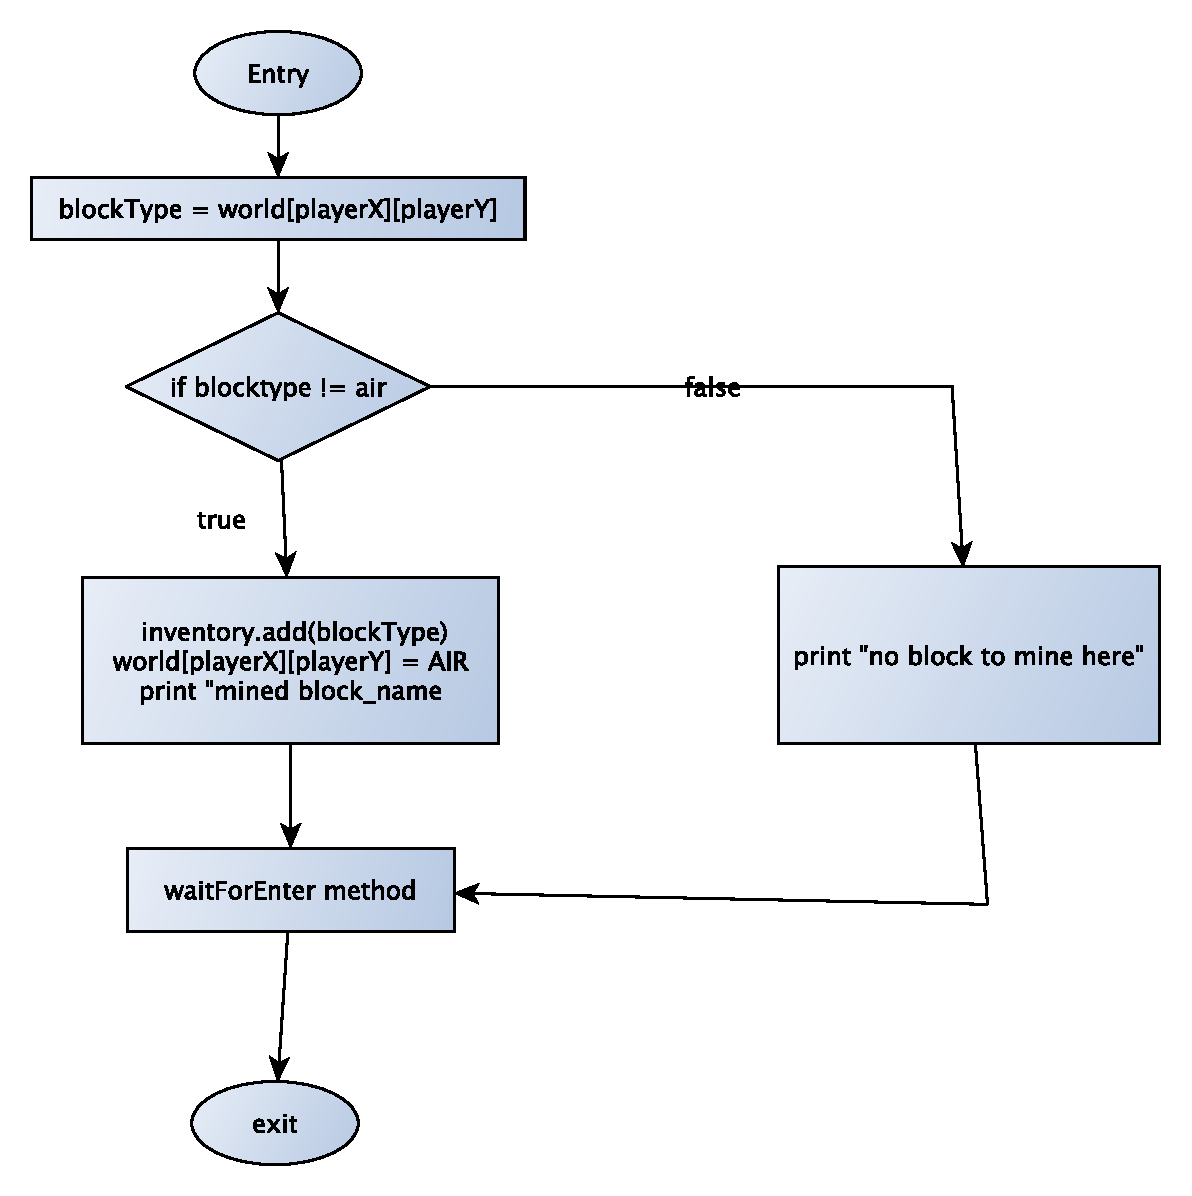
\includegraphics[width=\textwidth]{../flowchart/mineBlock.png}}
\begin{lstlisting}
function mineBlock()

blockType = world[playerX][playerY]
if blockType is not equal to AIR then 
	inventory.add(blockType)
	world[playerX][playerY] = AIR
	print("Mined " + getBlockName(blockType) + ".")
else print("No block to mine here.")
end if
waitForEnter()
end function
\end{lstlisting}
\newpage
{\includegraphics[width=\textwidth]{../flowchart/movePlayer.png}}
\begin{lstlisting}
function movePlayer(direction):

direction = uppercase(direction) //converts direction to uppercase for consistency
switch(direction):
case "W" or "UP":
	if playerY > 0 then playerY = playerY - 1
	end if
case "S" or "DOWN":
	if playerY < worldHeight - 1 then playerY = playerY + 1
	end if
case "A" or "LEFT":
	if playerX > 0 then playerX = playerX - 1
	end if
case "D" or "RIGHT":
	if playerX < worldWidth - 1 then playerX = playerX + 1
	end if
default: //do nothing
end switch
end function
\end{lstlisting}
\newpage

{\includegraphics[width=\textwidth]{../flowchart/fillInventory.png}}
\begin{lstlisting}
fillInventory()
Set INVENTORY_SIZE = 100

Clear inventory
FOR blockType = 0; blockType <= 4; blockType ++:
   FOR i = 0; i < INVENTORY_SIZE; i++:
      add block blockType to inventory
      
end function
\end{lstlisting}
\newpage
{\includegraphics[width=\textwidth]{../flowchart/generateEmptyWorld.png}}
\begin{lstlisting}
function generateEmptyWorld()

Set 2d array world = new int[NEW_WORLD_WIDTH][NEW_WORLD_HEIGHT]
Set redBlock = 1
Set whiteBlock = 4
Set blueBlock = 3
Set stripHeight = NEW_WORLD_HEIGHT / 3

FOR y = 0; y < stripHeight; y++:
    FOR x = 0; x < NEW_WORLD_WIDTH; x++:
        world[x][y] = redBlock

FOR y = stripHeight; y < stripHeight * 2; y++:
    FOR x = 0; x < NEW_WORLD_WIDTH; x++:
        world[x][y] = whiteBlock

FOR y = stripHeight * 2; y < NEW_WORLD_HEIGHT; y++:
    FOR x = 0; x < NEW_WORLD_WIDTH; x++:
        world[x][y] = blueBlock
end function
\end{lstlisting}
\newpage
{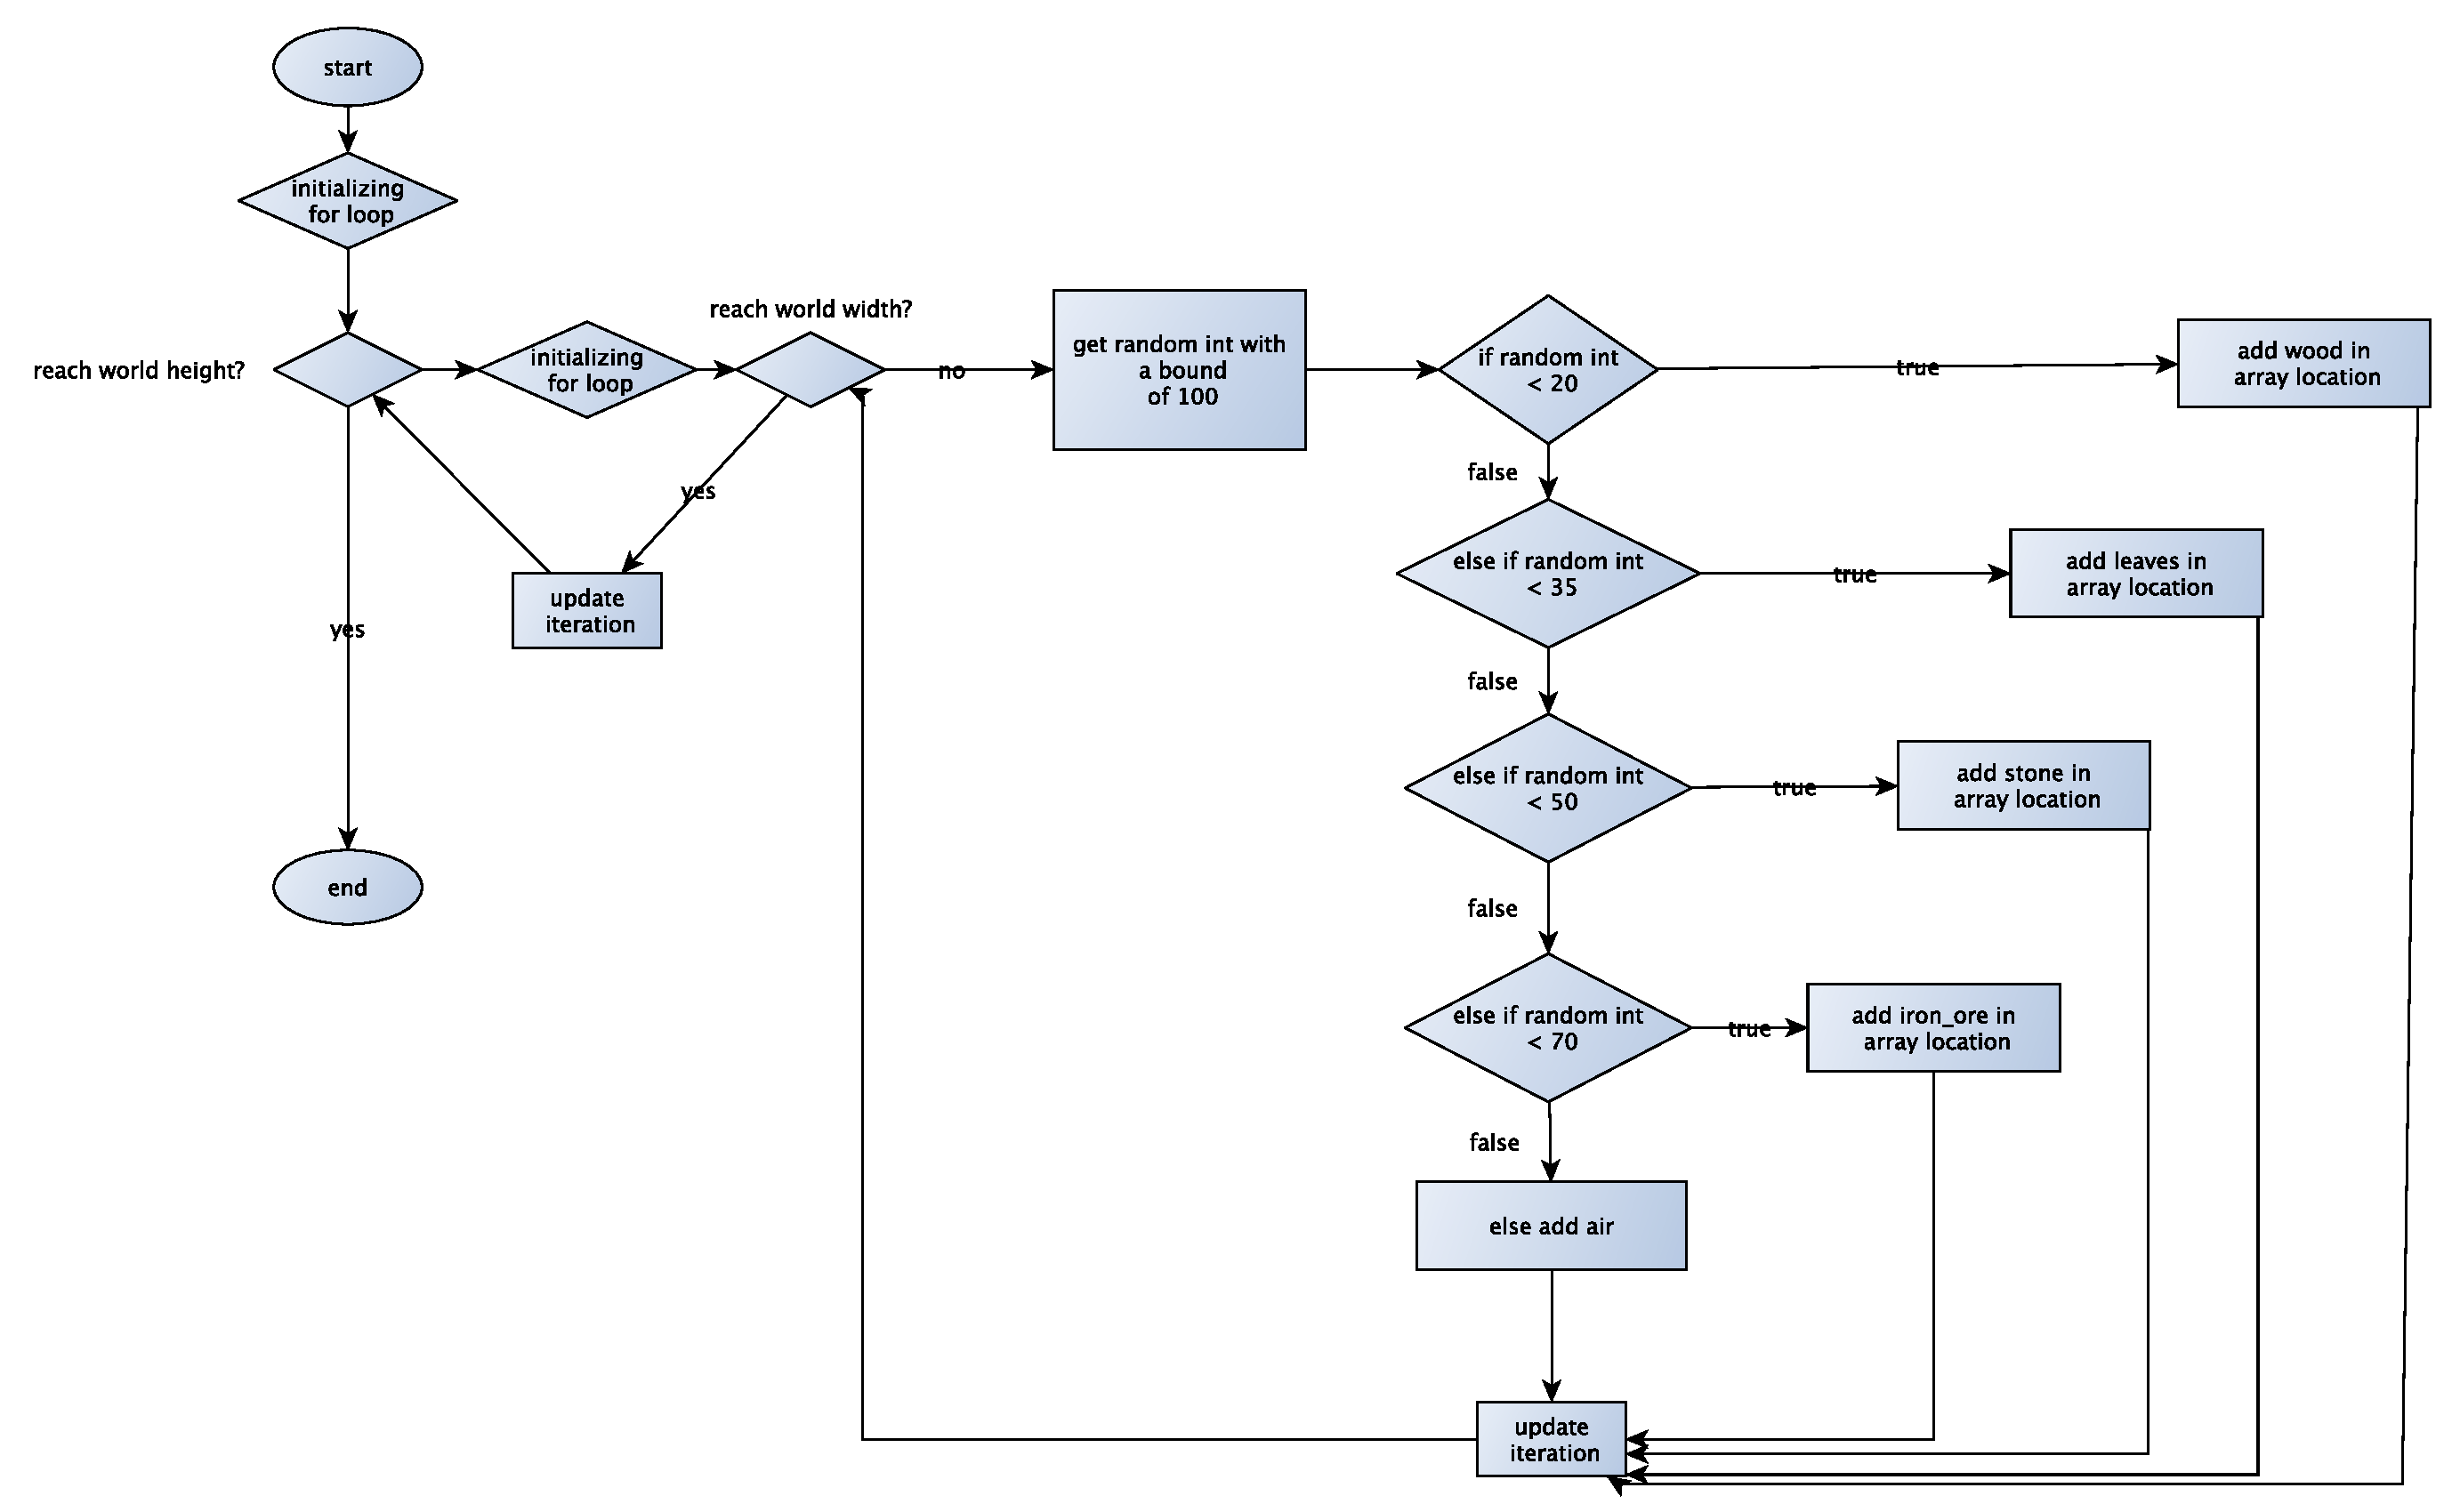
\includegraphics[width=\textwidth]{../flowchart/generateWorld.png}}
\begin{lstlisting}
function generateWorld()

FOR y = 0; y < WORLD_HEIGHT; y++:
  FOR x = 0; x < WORLD_WIDTH; x++:
    creates random number between 1 and 100
    if random number < 20
      creates wood at x, y
    else if random number < 35
      creates leaves at x, y
    else if random number < 50
      creates stone at x, y
    else if random number < 20
      creates iron ore at x, y
   else create air at x, y
end function
\end{lstlisting}
\newpage
{\includegraphics[width=\textwidth]{../flowchart/initGame.png}}
\begin{lstlisting}
function initGame()

Set worldwidth
Set worldheight
Set world = [worldwidht][worldheight]
Set playerx = worldwidght / 2
Set playery = worldheight / 2
Creates array list inventory

\end{lstlisting}
\newpage
{\includegraphics[width=\textwidth]{../flowchart/lookAround.png}}
\begin{lstlisting}
function lookAround()
Set playerX be x position of player
Set playerY be y position of player

print("You look around and see:")
FOR y = Math.max(0, playerY - 1); y <= Math.min(playerY + 1, worldHeight - 1); y++:
  FOR x = Math.max(0, playerX - 1); x <= Math.min(playerX + 1, worldWidth - 1); x++:
    if x == playerX and y == playerY:
      print("P");
    else:
      print(block at position [x][y])
  print empty line
print empty line
end function
\end{lstlisting}
\newpage

{\includegraphics[width=\textwidth]{../flowchart/getCountryAndQuoteFromServer.png}}

\begin{lstlisting}
  function getCountryAndQuoteFromServer():
  TRY:
  Set link = "https://flag.ashish.nl/get_flag"
  Setup a connection to link
  Set request method of connection to "POST"
  Set request property of connection to "Content-Type" as json
  Enable output of connection
  
  let payload be stringified json
  let writer be OutputStreamWriter of connection
        Write payload to writer
        Flush writer
        Close writer
        
        let reader be BufferedReader of connection
        let sb be StringBuilder
        let line be empty string
        WHILE (line is not null):
        let line read next line of reader
        Append line line to sb
            json = ConvertToString(sb)
            
            let countryStart = FindSubstringIndex(json, " ") + 11
            let countryEnd = FindSubstringIndex(json, " ", countryStart)
            let country = Substring(json, countryStart, countryEnd)
            
        let quoteStart = FindSubstringIndex(json, " ") + 9
        let quoteEnd = FindSubstringIndex(json, " ", quoteStart)
        let quote = Substring(json, quoteStart, quoteEnd)
        
        quote = ReplaceSpaces(quote)
        Print("Country: " + country)
        Print("Quote: " + quote)
        CATCH Exception AS e:
        stackTrace = GetStackTrace(e)
        Print("Error connecting to the server")
        Print(stackTrace)
        end function
\end{lstlisting}

{\includegraphics[width=\textwidth]{../flowchart/displayInventory.png}}
\begin{lstlisting}
  function displayInventory:

 print "Inventory"
 if inventory.isEmpty
    print ANSI_YELLOW + " empty" + ANSI_RESET 

else:
   make a 1D array blockCounts of size 5 
   for int i = 0; i < inventory.size(); i++
   int block = inventory.get(i) 
   blockCounts[block] 

For int blockType = 1; blockType < blockCounts.length; blockType++ 
   int occurrences = blockCounts[blockType] 
If occurrences > 0: 
   Print getBlockName(blockType) + " - " + occurrences
print "Crafted Item"
if craftedItems is null or craftedItems is empty
   print ANSI_YELLOW_ + "none" + ANSi_RESET
else 
   for int item : crafted item 
   print getCraftedItemColor(item) + getCraftedItemName(item) + ", " + ANSI_RESET

\end{lstlisting}

{\includegraphics[width=\textwidth]{../flowchart/getBlockName.png}}

\begin{lstlisting}
Function getBlockName(blockType):

Switch blockType 
Case AIR:
 Return "Empty Block" 
Case WOOD: 
Return "Wood" 
Case LEAVES: 
Return "Leaves" 
Case STONE: 
Return "Stone"
 Case IRON_ORE: 
Return "Iron Ore" 
Default:
 Return "Unknown" 

\end{lstlisting}

{\includegraphics[height=\textheight]{../flowchart/loadGame.png}}

\begin{lstlisting}
  Function loadGame(fileName) 
Try Create ObjectInputStream inputStream using FileInputStream(fileName) 
load NEW_WORLD_WIDTH from inputStream 
load NEW_WORLD_HEIGHT from inputStream 
load world from inputStream as a 2D integer array 
load playerX from inputStream 
load playerY from inputStream 
load inventory from inputStream as a list of integers 
load craftedItems from inputStream as a list of integers 
load unlockMode from inputStream 
Print "Game state loaded from file: " + fileName
 Catch IOException or ClassNotFoundException e 
Print "Error while loading the game state: " + e.getMessage() 

\end{lstlisting}
{\includegraphics[width=\textwidth]{../flowchart/removeItemsFromInventory.png}}
\begin{lstlisting}
function removeItemsFromInventory(item, count):

removedCount = 0 
iterator = createIterator(inventory) 
While iterator.hasNext()
    i = iterator.next() 
If i is equal to item iterator.remove() 
   removedCount = removedCount + 1 
If removedCount is equal to count
    break
\end{lstlisting}

{\includegraphics[height=\textheight]{../flowchart/saveGame.png}}

\begin{lstlisting}
  function saveGame(fileName):

Try  ObjectOutputStream outputStream
 save NEW_WORLD_WIDTH to outputStream 
save NEW_WORLD_HEIGHT to outputStream
 save world to outputStream 
save playerX to outputStream
 save playerY to outputStream
 save inventory to outputStream 
save craftedItems to outputStream 
save unlockMode to outputStream
 Print "Game state saved to file: " + fileName Catch IOException e 
Print "Error while saving the game state: " + e.getMessage() 

\end{lstlisting}


\newpage

\end{document}
